\documentclass[egregdoesnotlikesansseriftitles,a4paper,fontsize=12pt]{scrartcl}
\usepackage{graphicx}
\usepackage{microtype}
\usepackage{scrextend}
\usepackage[utf8]{inputenc}
\usepackage[czech]{babel}
\usepackage{librebaskerville}
\usepackage[T1]{fontenc}

\begin{document}
\begin{center}
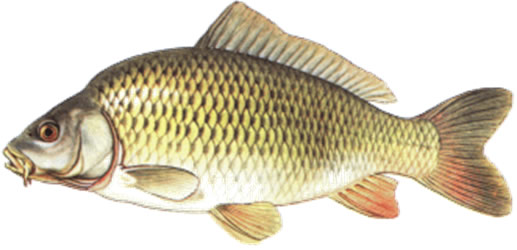
\includegraphics[width=.5\linewidth]{kapr-obecny-kresba.jpg}\\[1em]
\huge{\textsc{Pravidla rybaření na rybníku Spáleniště}}\\
\end{center}
\vspace{6em}

Rybáři ubytování v našem penzionu oceňují klid, pořádek, nenarušené okolí
rybníka a čistotu. Aby se jim u rybníka líbilo i v budoucnu, je nezbytné, aby
každý rybář zachovával pořádek a šetrně a ohleduplně se choval k přírodě. K tomu napomůže dodržování těchto pravidel:
\begin{itemize}
\item Nezasahujeme do okolní přírody, např. neřežeme
vidličky z rostoucích
stromů.
\item Škrábání, kuchání a porcování ryb neprovádíme u rybníka a v jeho okolí.
\item Po ukončení rybolovu uklidíme místo tak, aby vypadalo jako při našem příchodu.
\item U rybníka a v jeho okolí nerozděláváme oheň.
\item Veškeré odpadky odnášíme s sebou.
\end{itemize}

Lov ryb smí být prováděn jen způsobem odpovídajícím zásadám řádného výkonu
rybářského práva, ochrany ryb a ostatních vodních živočichů. S ulovenými rybami
je rybář povinen zacházet šetrně a dle rybářské etiky, zejména je nepoškozovat
vláčením po břehu, násilným vyprošťováním zaseknutých háčků a trýznit
ponecháním na suchu.
\pagebreak

\section*{Rybářské nářadí, způsob lovu a nástrahy}
\begin{itemize}
\item Je povoleno chytat na dva pruty, každý s max. jedním návazcem s jednoduchým háčkem.
\item Při přívlači je dovoleno lovit jen jedním prutem s jedním návazcem, přičemž nesmí být další pruty nastraženy.
\item Muškaření je dovoleno jen jedním prutem, nejvýše se dvěma návazci a nesmí být nastraženy další pruty.
\item Lov na přívlači, nebo lov na živou či mrtvou rybku je povolen v době od 16.6. do 31.12.
\item Rybolov mládeže do 15 let: lovící smí použít k lovu pouze 1 prut.
\item Je zakázáno vnadit krví, neuvařeným partiklem, luštěninami, arašídy, ořechy, boby, masem a směsmi z masa, bílými červy, mlékárenskými kaly, škrkavkami, i všemi živočichy chráněnými zákonem včetně jejich vývojových stádií.
\item Při lovu je rybař povinen mít: vyprošťovač háčků, pevnou míru (metr), podběrák, pean, podložku pod ryby a vezírek s pevnými  kruhy
\item Je striktně zakázáno lovit na srkačku, čeřenem, i s použitím samoseku.
\item V případě fotodokumentace je nutné rybu fotit nad podložkou a v bezpečné výšce.
\end{itemize}

\pagebreak
\section*{Ceny povolenek}
\begin{labeling}{Dětská\quad}
    \item[Denní] 400,-- Kč systém chyť a pusť. Rybu je možno po dohodě s majitelem odkoupit, za předem dohodnutých podmínek.
    \item[Dětská] \textit{Cena dohodou}
\end{labeling}

\section*{Denní doby lovu}
\begin{labeling}{leden, únor, listopad a prosinec\quad}
\item[Květen--srpen] 04--24 hod
\item[Březen, duben, září a říjen] 06--22 hod
\item[Leden, únor, listopad a prosinec] 07--18 hod
\item[Noční lov] \textit{Po domluvě}
\end{labeling}

\section*{Lovné míry ryb}
\begin{labeling}{Tolstolobik\quad}
    \item[Kapr] 45--65 cm
    \item[Amur] 50--60 cm
    \item[Tolstolobik] 60--80 cm
    \item[Štika] 60--80 cm
    \item[Lín] \textit{Lov zakázán}
\end{labeling}
Ostatní ryby vracíme zpět vodě.

\end{document}
